\chapter{Analysis}
\label{ch:anal}

\section{TMTO Attack}
As the keysize of an attack on the KASUMI cipher used in the 2G
network is \code{64-bit}, we have to perform our tests on a scaled down
key. With the hardware at our disposal the computation of a table
required to perform the attack on a \code{64-bit} key would simply be
unrealistic. Therefore all of our testing is done on tables generated
with \code{32-bit} keys. We use the same idea as the scaling from \code{128-bit} to
\code{64-bit} discussed in chapter \ref{ch:kas}.

Thus a key $K$ built from a \code{32-bit} $K_{32} = K_1 || K_2$  implementation will
look as follows
\[K = K_1 || K_2 || K_1 || K_2 || K_1 || K_2 || K_1 || K_2\]
As to gain an idea of how our implementation matches up with
the math and parameter choices done in chapter \ref{ch:param}, we have to generate
information on an actual attack on a \code{32-bit} key. If the \code{32-bit} test
results match with our calculations, we can begin to give estimates
on the actual attack(\code{64-bit} keysize).
\subsection{Pre-computational phase}
To test the table generation we will first set some parameters
valid for \code{32-bit} testing.

Using the same parameter setup as described in \ref{sec:rainbowparam}
table \ref{tab:rainparam32} gives us valid parameter choices. For the
testing of \code{32-bit} no boundaries were set.
\begin{table}[H]
  \centering
  \text{\texttt{Success{ }={ }0.730000,{ }Rmsc{ }={ }1.849002,{ }l{ }={ }1,{ }Offline{ }phase{ }={ }2{\char`\^}32.886747}}
  \begin{tabular}{llll}
    m & t & M(MB) & T \\ \hline
    $2^{25.00}$ & $2^{7.89}$ & $134.22$ & $2^{13.67}$ \\
    $2^{25.50}$ & $2^{7.39}$ & $189.81$ & $2^{12.71}$ \\
    $2^{26.00}$ & $2^{6.89}$ & $268.44$ & $2^{11.76}$ \\
    $2^{26.50}$ & $2^{6.39}$ & $379.63$ & $2^{10.83}$ \\
    $2^{27.00}$ & $2^{5.89}$ & $536.87$ & $2^{9.92}$ \\
  \end{tabular}
  \caption{Rainbow Parameters - 32-bit keysize}
  \label{tab:rainparam32}
\end{table}
Since we are only testing on \code{32-bit} there is no real concern of
memory usage or online time. For this reason we went with a parameter
choice of $m=2^{25} \approx 33445532$ and $t= 2^{7.89} \approx
236$. The table generator will be tested on the actual
pre-computational time and the memory usage.
\subsubsection{Pre-computational time}
Table \ref{tab:rainparam32} states that an expected amount of
KASUMI encryptions required for generation of the table is
$2^{32.886}$. Looking back to \ref{sec:benchkas} we know the
amount of time it takes our test machines to perform 10000000 encrytions. As an
example the previously mentioned Zenbook i7 is used. The
Zenbook will perform 10000000 KASUMI encryptions in 1,897
seconds. From this we get an idea of how many encryptions our
machine execute in 1 second.
\[10000000 enc / 1.897 s = 5291005,29 \quad enc/s\]
Now we can calculate the expected running time of the
pre-computational phase
\[2^{32.886} / 5291005.29 \approx 1500s = 25 min \]
Running our implementation with UNIX-command
\code{time}\footnote{\url{https://en.wikipedia.org/wiki/Time_(Unix)}}
allows us to easily check whether or not this matches up. Running the
implementation multiple times resulted in average running time of
approximately 27 minutes. This is $\approx8\%$ more time used than
expected. This can be seen as expected as time is required to write
the table to a disk. Another explanation could be our sequential
approach and the usage of the MD5 algorithm. TODO Some facts to back up maybe?
\subsubsection{Memory}
We also want to make sure that the actual memory usage matches up with
the expected. From our parameter choice we can see the expected memory
$M_{predicted}=134.22$MB. The previously generated table can easily be
checked to make sure this is correct. Using the UNIX-command
\code{wc}\footnote{\url{https://en.wikipedia.org/wiki/Wc_(Unix)}} with
the \code{-c} flag will allow us to get the byte count of the
generated binary file. Performing this command on our generated table
unsurprisingly gave us a result of
$M_{actual}=134217728\text{B}\approx134.22$MB.

Knowing the time usage and memory usage in the pre-computational phase
matches up with our expected values, we can now give an approximate of
how scaling from a \code{32-bit} keysize to a \code{64-bit} keysize
will look.

Again we take a look back to \ref{sec:rainbowparam}. As we are now
dealing with the actual \code{64-bit} attack the boundaries we set
will now be taken into account again. From the tests on the
\code{32-bit} implementation we saw the size of the table match up
perfectly. Because of this we will not discuss table size further, as
adding additional bit to a binary file should not change the outcome.
Going with the parameters chosen in \ref{sec:rainbowparam} we set
$m=?$ and $t=?$.
\subsubsection{Scaling to 64-bit keysize}
From the chosen parameters we know that the pre-computational phase is
estimated to require $2^{64.88}$ encryptions of KASUMI. This amount of encryptions
is infeasible to run on the devices that we ran the
\code{32-bit} implementation on. Thus for generating a table of that
size a server/cluster with a huge amount of processing power is
required. As an example we will try to give some rough estimates on
how much computational power is needed and how many cores this would
translate to.

We will try to give an estimate, from our tests, to a table generated
in roughly 24 months. This was chosen as any faster would essentially
require more processing power than could be expected from even some the
fastest super computers
today\footnote{\url{http://www.top500.org/lists/2014/11/}}. First off
we know from \ref{tab:zen} that for 1 encryption of
\code{64-bit} of data, we need to use $68,76 * 8 \approx 550$ CPU
cycles. 

From the pre-computational time noted earlier we can now estimate how
many cycles will be needed to compute all encryptions required.
\[ cycles_{tot} = 550 * 2^{64.88} \approx 2^{74}\]
From this we can estimate the required cycles per second a build needs
to do. 
\[ cycles_{sec} = \frac{2^{74}}{550} \approx 2^{48}\]
This translates to a frequency of around  \code{295887Ghz}. Looking at
highend server cores for clusters, they might have a maximal frequency
of around\code{4,4ghz} per core. If we expect every core can perform
equally and perform at this frequency we would need $\approx 67000$
cores to generate the table in two years.


\subsection{Online phase}
\subsubsection{Time}
As stated earlier are the tests preformed on a scaled down version of the keyspace.
The tests are run on the 32 bit implementation and then scaled up.
Firstly the Time it takes is compared to our computations, as Time is found by $Time=\frac{t\cdot(t-1)}{2}$.
Table\ref{tab:OnlineT} shows each of our test tables worst case run times and the calculated encryption time for each of them.
Each  table has an online encryption time spanning from a few miliseconds to a few microseconds, wheras the total time is  much larger.
Furthermore if we don't add in the fact that the computer is smart and caches memory it takes even longer, which is shown in the T lookup field(this the time one lookup takes when it isn't in memory multiplied with t which is the amount of lookups).
\begin{table}[H]
\centering
\caption{Online Time Comparison}
\label{tab:OnlineT}
\begin{tabular}{|c|ccccc}
\hline
Table          & \multicolumn{1}{c|}{t rounded up} & \multicolumn{1}{c|}{Total time} & \multicolumn{1}{c|}{T lookup} & \multicolumn{1}{c|}{T enc} & \multicolumn{1}{c|}{encryptions} \\ \hline
134MB / 73\%   & 236                           & 7.5995 s                        & 7.972375 s                    & 5.24E-03 s                 & 27,730.00                        \\ \cline{1-1}
4300MB / 73\%  & 8                             & 27.339 s                        & 36.724 s                      & 5.29E-06 s                 & 28.00                            \\ \cline{1-1}
8500MB / 73\%  & 4                             & 73.35 s                         & 67.196 s                      & 1.13E-06 s                 & 6.00                             \\ \cline{1-1}
12000MB / 73\% & 3                             & 70.97 s                         & 69.811 s                      & 5.67E-07 s                 & 3.00                             \\ \cline{1-1}
17000MB / 73\%  & 2                             & 66.96 s                         & 65.11 s                       & 1.89E-07 s                 & 1.00                             \\ \cline{1-1}
\end{tabular}
\end{table}
This means that the biggest bottleneck in the implementation is the lookup time. To further investigate this we calculate the lookup time for each table, and compare them to each other note that the test computer has a max read speed of 540 mb/s. One thing we noticed is when the entire table can fit in memory the access time of it increases dramatically, for the 4.3GB table the first table lookup took 4.4 seconds and the lookups afterwards took between 0.6-1 seconds. This is probably due to the table getting cached.
\begin{table}[h]
\centering
\caption{Access time}
\label{tab:memory}
\begin{tabular}{|c|clccc}
\hline
\multicolumn{1}{|l|}{Buffer-size$\downarrow$ Table-size$\rightarrow$}& \multicolumn{1}{c|}{134MB} & \multicolumn{1}{l|}{4300MB} & \multicolumn{1}{c|}{8500MB} & \multicolumn{1}{c|}{12000MB} & \multicolumn{1}{l|}{17000MB} \\ \hline
33554432                                     & 0.0427s                    & 4.4395s                     & 16.829s                     & 23.230s                      & 32.562s                      \\ \cline{1-1}
524288                                       & 0.023s                     & 4.4395s                     & 16.645s                     & 23.279s                      & 32.72s                       \\ \cline{1-1}
65536                                        & 0.021s                     & 4.4585s                     & 16.941s                     & 23.002s                      & 32.483s                      \\ \cline{1-1}
32                                           & 0.053s                     & 5.0245s                     & 16.780s                     & 23.57s                       & 32.44s                       \\ \cline{1-1}
\multicolumn{1}{|l|}{Scaled to 8 tb table}   & 0.6 Hours                  & 2.37 Hours                  & 4.45 Hours                   & 4.31 Hours                   & 4.25 Hours                   \\ \cline{1-1}
\end{tabular}
\end{table}
As \ref{fig:memory} shows the buffer size does not seem to matter much the results fluxuates half a second at most.
The table also shows what the lookup time would be if the table was 8 tb. Where target table size is tts, table size is ts, s is the time one lookup takes in seconds and 3600 is to get it in hours $\frac{\frac{tts}{ts/s}}{3600}$
\begin{figure}[H]
  \centering
  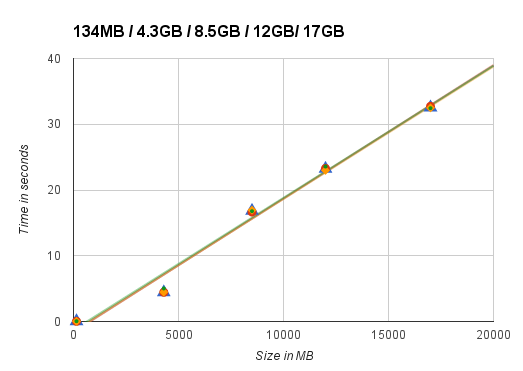
\includegraphics[width=0.8\textwidth]{figures/AccessTime.png}
  \caption{Access time for different table sizes and buffer sizes\\
    Green buffersize= 33554432 bit\\
    Red buffersize = 524288 bit\\
    Orange buffersize = 65536 bit\\
    Blue buffersize = 32 bit\\
    }
  \label{fig:tableAccess}
\end{figure}

Also something to note when scaling the access time up to a table that is 8tb the lookup time is around 4.2-4.45 hours.
One thing to note though is when the table is small enough to fit the
memory it gives faster results, which can be ignored since the entire
8 tb table does not fit memory. Now where the access time is estimated
we can give a approximation of the online phase for the \code{64-bit}
keyspace. As previously stated the access time would lie around
4.2-4.45 hours for each lookup, so for $m=2^{39.80}$ and $t=2^{25.08}$
this means that the lookup time comes to $t\cdot
lookupTime=2^{25.08}\cdot 4.45 Hours \approx 18,005 years$. The
Encryption time would be $2^{25.08}\cdot\frac{2^{25.08}-1}{2}\approx
\frac{6.2897672e+14 encryptions}{5291005 encryptions/sec} \approx 3.7
years$ so the online phase would approximately take $18008.7
years$. Which leads to the conclusion that our implementation would
not work in its current state. To get a more realistic attack we will
in section \ref{sec:Discussion} explain some memory optimizations and
the RainbowDP table that reduces the amount from t to 1. To get the
encryption time down to approximately one day one would need 1280
cores.

\subsubsection{Table Coverage}

If the attack should be able to be carried out in a real-world
scenario, we need to make sure the predicted table coverage matches up
with the results from our implemenation. These tests can only be done
on our \code{32-bit} implementation of the attack. If the results
matches up with the expected, we can assume that our table is
generated correctly. We also have to assume that if the results
matches up for our \code{32-bit} implementation, they will also match
up for the \code{64-bit} implementation.

From \ref{tab:rainparam32} we know the table generated with the given
parameters should result in a success rate of $73\%$. We can therefore
expect the coverage of the table to be around $2^{32} * 0.73 =
2^{31.54}$. In some smaller test cases with a smaller keysize, we were
able to count how many distinct keys were in the table, but for
\code{32-bit} we found this way of counting too slow. Instead we tried
checking random keys to give an insight in how many keys we
actually covered. We checked keys until a somewhat stable distribution was
reached. Checking 100 random ciphers allowed us to give a pretty
reasonable idea of how the success probability would match up to the
actual coverage.

From running our online phase on a generated table with 100 random
generated ciphers, we found that $74\%$ of the ciphers found a
matching key in the table. This is well within the expected
distribution when only running 100 tests, and we can therefore expect
our table to cover $\approx73\%$ of the keyspace.




\section{Cost analysis}
In this section we will assume that the memory optimizations has been implemented and the table is of Rainbow/DP\ref{sec:Discussion}. This gives a table access of 1, when a DP is reached.
To pull this off for $m=2^{39.80}$ and $t=2^{25.08}$ the pre-computation will require \code{7.56TB}, and \code{$2^{64.88}$} encryptions. The online phase will require \code{$2^{49.16}$} encryptions, our cost analysis will aim at getting the online phases encryption time down to one day. This will require $\frac{2^{49.16}}{60*60*24}\approx 2^{32.76}$ encryptions per second. We have found a couple of candidates that fits the bill:

% Please add the following required packages to your document preamble:
% \usepackage[table,xcdraw]{xcolor}
% If you use beamer only pass "xcolor=table" option, i.e. \documentclass[xcolor=table]{beamer}
\begin{table}[H]
\caption{Hardware comparison}
\label{my-label}
\begin{tabular}{|ccccccc}
\hline
\rowcolor[HTML]{EFEFEF}
CPU                                    &                             &                               &                           &                                 &                            & \multicolumn{1}{l|}{\cellcolor[HTML]{EFEFEF}} \\ \hline
\multicolumn{1}{|c|}{Model}            & \multicolumn{1}{c|}{Cores}   & \multicolumn{1}{c|}{Amount} & \multicolumn{1}{c|}{Ghz}  & \multicolumn{1}{c|}{Enc per sec} & \multicolumn{1}{c|}{Price USD} & \multicolumn{1}{c|}{Total USD}                    \\ \hline
\multicolumn{1}{|l|}{AMD FX-8320}      & 8                            & 143                         & 3,5                       & 7278941245                      & 139                    & 20020                                     \\
\multicolumn{1}{|l|}{AMD FX-8350}      & 8                            & 125                         & 4                         & 7271669575                      & 170                   & 21250                                    \\ \hline
\rowcolor[HTML]{EFEFEF}
Hard Drive                                                          &                               &                           &                                 &                           & & \multicolumn{1}{l|}{\cellcolor[HTML]{EFEFEF}} \\ \hline
\multicolumn{1}{|c|}{Model}            & \multicolumn{1}{c|}{Size GB} & \multicolumn{1}{c|}{Amount} & \multicolumn{1}{c|}{Read $mb/s$} & \multicolumn{1}{c|}{Write $mb/s$}      & \multicolumn{1}{c|}{Price USD} & \multicolumn{1}{c|}{Total USD}                    \\ \hline
\multicolumn{1}{|c|}{Crucial}          & 960                          & 8                           & 500                       & 400                             & 300                        & 2400                                          \\
\multicolumn{1}{|c|}{Mushkin} & 1000                         & 8                            & 560                       & 460                             & 339                        & 2712                                          \\ \cline{1-1}
\end{tabular}
\end{table}
So with around $20020+2712=22732 $USD $ \approx 151313 $DK for the harddrive and the CPU's.

%%% Local Variables:
%%% mode: latex
%%% TeX-master: "Thesis"
%%% End:
